La imagen muestra las distancias en kilómetros entre tres ciudades.
Como se muestran a continuación en la figura \ref{fig:proverb_pitagoras_04}
\begin{figure}[H]
    \begin{center}
        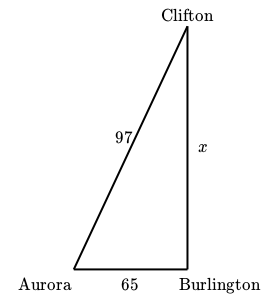
\includegraphics[width=0.25\linewidth]{../images/proverb_pitagoras_04.png}
    \end{center}
    \caption{}
    \label{fig:proverb_pitagoras_04}
\end{figure}
\textbf{¿Qué tanto más corto es viajar directamente de Aurora a Clifton que de Aurora a Clifton pasando por Burlington?}\\

\begin{solutionbox}{12cm}
    Podemos usar el teorema de Pitágoras para obtener $x$.
    La ecuación del teorema de Pitágoras es:
    \[c^2=a^2+b^2\]
    donde $a$ y $b$ son las longitudes de los dos catetos del triángulo y $c$ es la longitud de la hipotenusa.
    En este caso, $a=65$, $b=x$ y $c=97$.
    \begin{align*}
        97^2         & =65^2+x^2     \\
        9,409        & = 4,225 + x^2 \\
        9,409-4,225  & =x^2          \\
        5,184        & =x^2          \\
        \sqrt{5,184} & =x            \\
        72           & = x
    \end{align*}
    Para calcular qué tan lejos es viajar a Clifton pasando por Burlington, podemos sumar las distancias entre cada una de las ciudades.
    \[65+72=137\]
    Para calcular qué tanto más corto es viajar directamente a Clifton, podemos restar.
    \[197-97=40\]
    Viajar directamente de Aurora a Clifton es 40 kilómetros más corto.
\end{solutionbox}